\documentclass[10pt,twocolumn, letterpaper]{article}

\usepackage{cvpr}
\usepackage{times}
\usepackage{epsfig}
\usepackage{graphicx}
\usepackage{amsmath}
\usepackage{amssymb}
\usepackage{kotex}
\usepackage{pifont}

\newcommand*\OK{\checkmark}
\newcommand*\BOLDOK{\ding{51}}

% Include other packages here, before hyperref.

% If you comment hyperref and then uncomment it, you should delete
% egpaper.aux before re-running latex.  (Or just hit 'q' on the first latex
% run, let it finish, and you should be clear).
\usepackage[breaklinks=true,bookmarks=false]{hyperref}

\cvprfinalcopy % *** Uncomment this line for the final submission

\def\cvprPaperID{****} % *** Enter the CVPR Paper ID here
\def\httilde{\mbox{\tt\raisebox{-.5ex}{\symbol{126}}}}

% Pages are numbered in submission mode, and unnumbered in camera-ready
%\ifcvprfinal\pagestyle{empty}\fi
\setcounter{page}{1}
\begin{document}

%%%%%%%%% TITLE
\title{Final Project. CAPTCHA Image Recognition using CNN and LSTM}

\author{Sangjun Son\\
Seoul National University\\
Department of Computer Science and Engineering\\
{\tt\small lucetre@snu.ac.kr}
}

\maketitle

\section{Introduction}

Everyone hates CAPTCHAs — those annoying images that contain text you have to type in before you can access a website \cite{captcha}. A CAPTCHA (an acronym for "Completely Automated Public Turing test to tell Computers and Humans Apart") is a type of challenge–response test used in computing to determine whether or not the user is human \cite{recaptcha}. It is to prevent computers from automatically filling out forms by verifying that you are not a robot. But with the rise of deep learning and computer vision, decoding CAPTCHA seems to be possible and some of those systems are even more better than human.

Given an image, how can we recognize characters from the CAPTCHA image? Since each CAPTCHA image has a variable length of characters, considering length will be a significant work while training through deep neural networks. If we can split the image apart so that that each letter is a separate image, remaining work is just to train the neural network to recognize a single letter at a time\cite{captcha}.

We've trained our network with 10,000 training examples whose lengths are in 2 $\sim$ 5 and tested with 1,000 test images of length 2 $\sim$ 7. Due to several parameters consisting the ensemble model of CNN and LSTM, we've conduct various experiments. After several experiments, we've found the best set of hyper-parameters that make our model perform more accurately and even faster.

\begin{center}
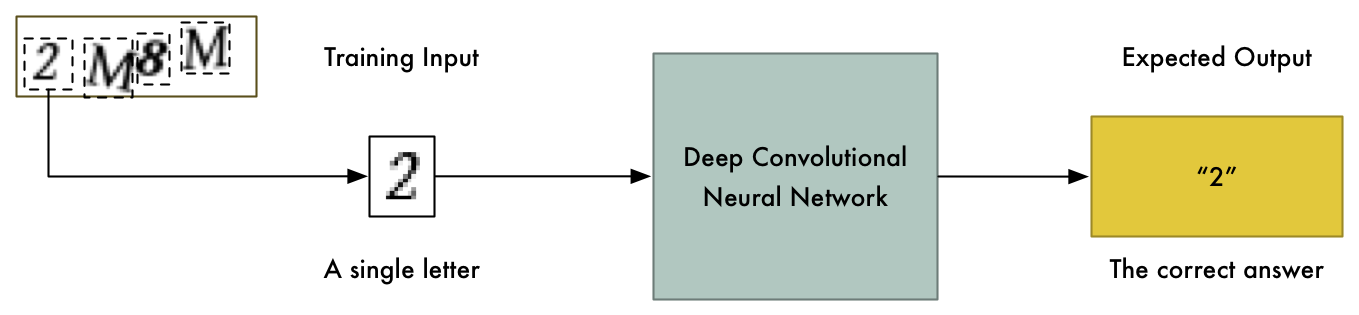
\includegraphics[width=1\linewidth]{./overview.png}
\end{center}

%-------------------------------------------------------------------------
\section{Related Works}

CATCHA recognition is one part of temporal pattern recognition projects. Simiarly, there are numerous examples like image captioning, speech recognition, part-of-speech tagging. Using ResNet and LSTM modules, which are the representatives of CNN and RNN methods, we can extract useful features from an image and continuously learning them over time.

%-------------------------------------------------------------------------
\section{Proposed Method}
This section describes overall flows of our proposed method, \texttt{BetterNet+LSTM}. Feature extraction and learning the temporal patterns are the key concepts of our model.

\begin{center}
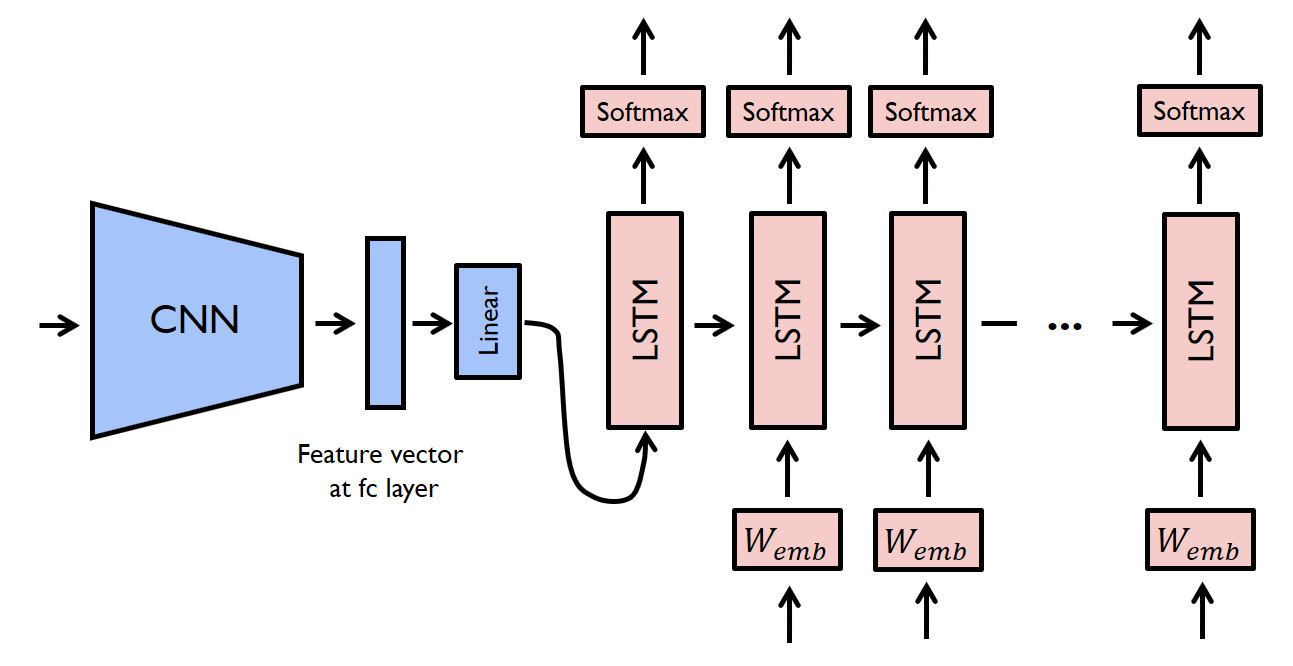
\includegraphics[width=1\linewidth]{./model.jpg}
\end{center}

\subsection{Feature extraction by BetterNet}
Since image vectors contain lots of information, we have to extract meaningful features. There exist lots of models like AlexNet, GoogLeNet and so on. We've implemented our own CNN module, but it showed too much low performance since it has few parameters for feature extraction due to shallow depth. \texttt{BetterNet} based on ResNet has been chosen to be our optimal CNN model. Comparison between our old model and \texttt{BetterNet} shows remarkable model complexity gap.

\begin{center}
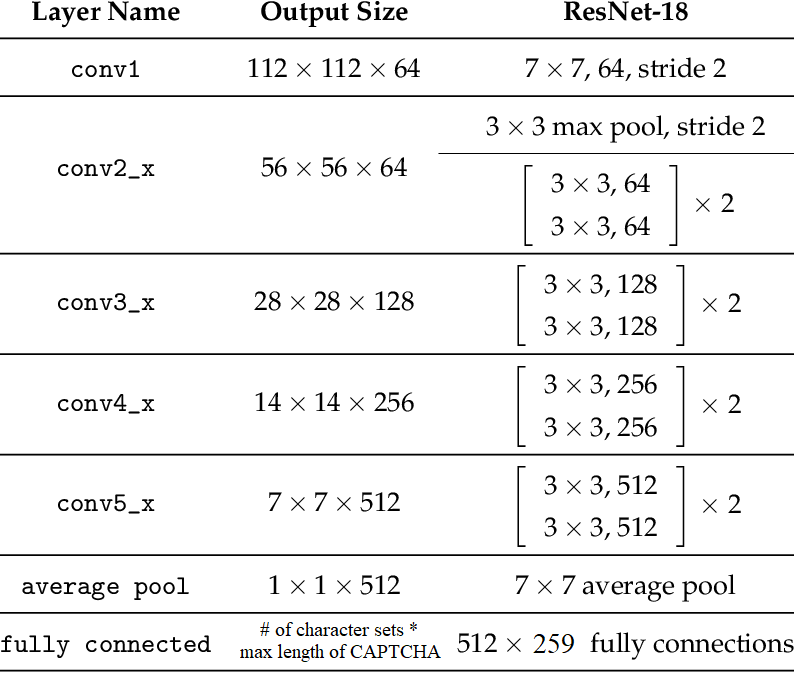
\includegraphics[width=1\linewidth]{./resnet18.png}
\end{center}

\subsection{Learning temporal patterns by LSTM}
The pretrained CNN extracts the feature vector from a given input image. The feature vector is linearly transformed to have the same dimension as the input dimension of the LSTM network. Using these source and target sequences and the feature vector, the LSTM decoder is trained as a language model conditioned on the feature vector \cite{image-captioning}. Putting together, our model \texttt{BetterNet+LSTM} was trained by Adam: A Method for Stochastic Optimization\cite{adam} with learning rate of 0.01 and maximum iteration of 200. \texttt{BetterNet+LSTM} shows fast and accurate performance of 303 sec as training time and 1.99e-4 as training multi-label loss. After testing 1,000 images, both character and word correctness of our model were 100.0\%.

\begin{center}
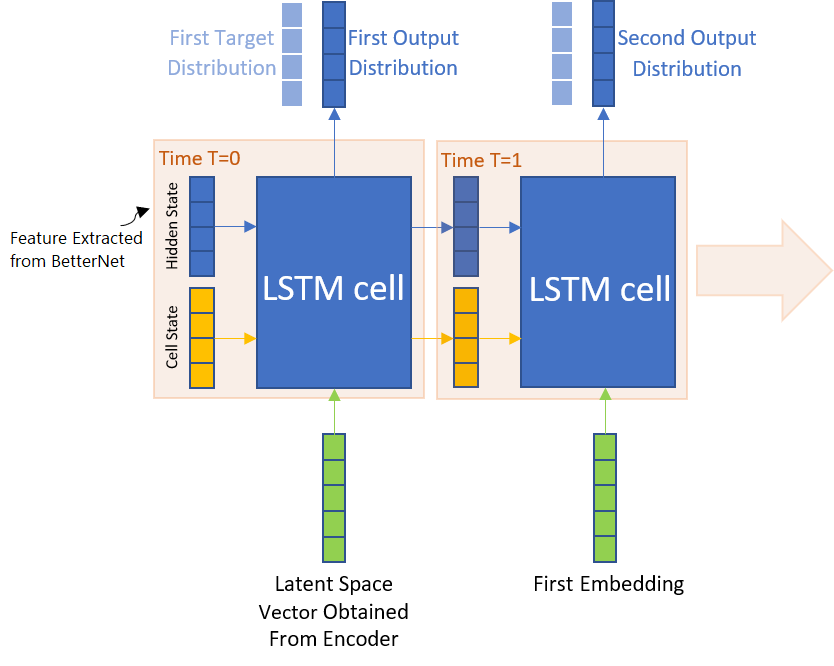
\includegraphics[width=1\linewidth]{./lstm.png}
\end{center}

%-------------------------------------------------------------------------
\section{Empirical Analysis}

Here we describes how we came up with \texttt{BetterNet+LSTM} model. Comparison analysis of \texttt{ResNet} and \texttt{BetterNet+LSTM} in aspect of time and accuracy in training is as the figure below. Both were trained by ADAM method with the same tolerance, maximum number of iterations and the learning rate of 1e-4, 200, 1e-2 \wrt.

\begin{center}
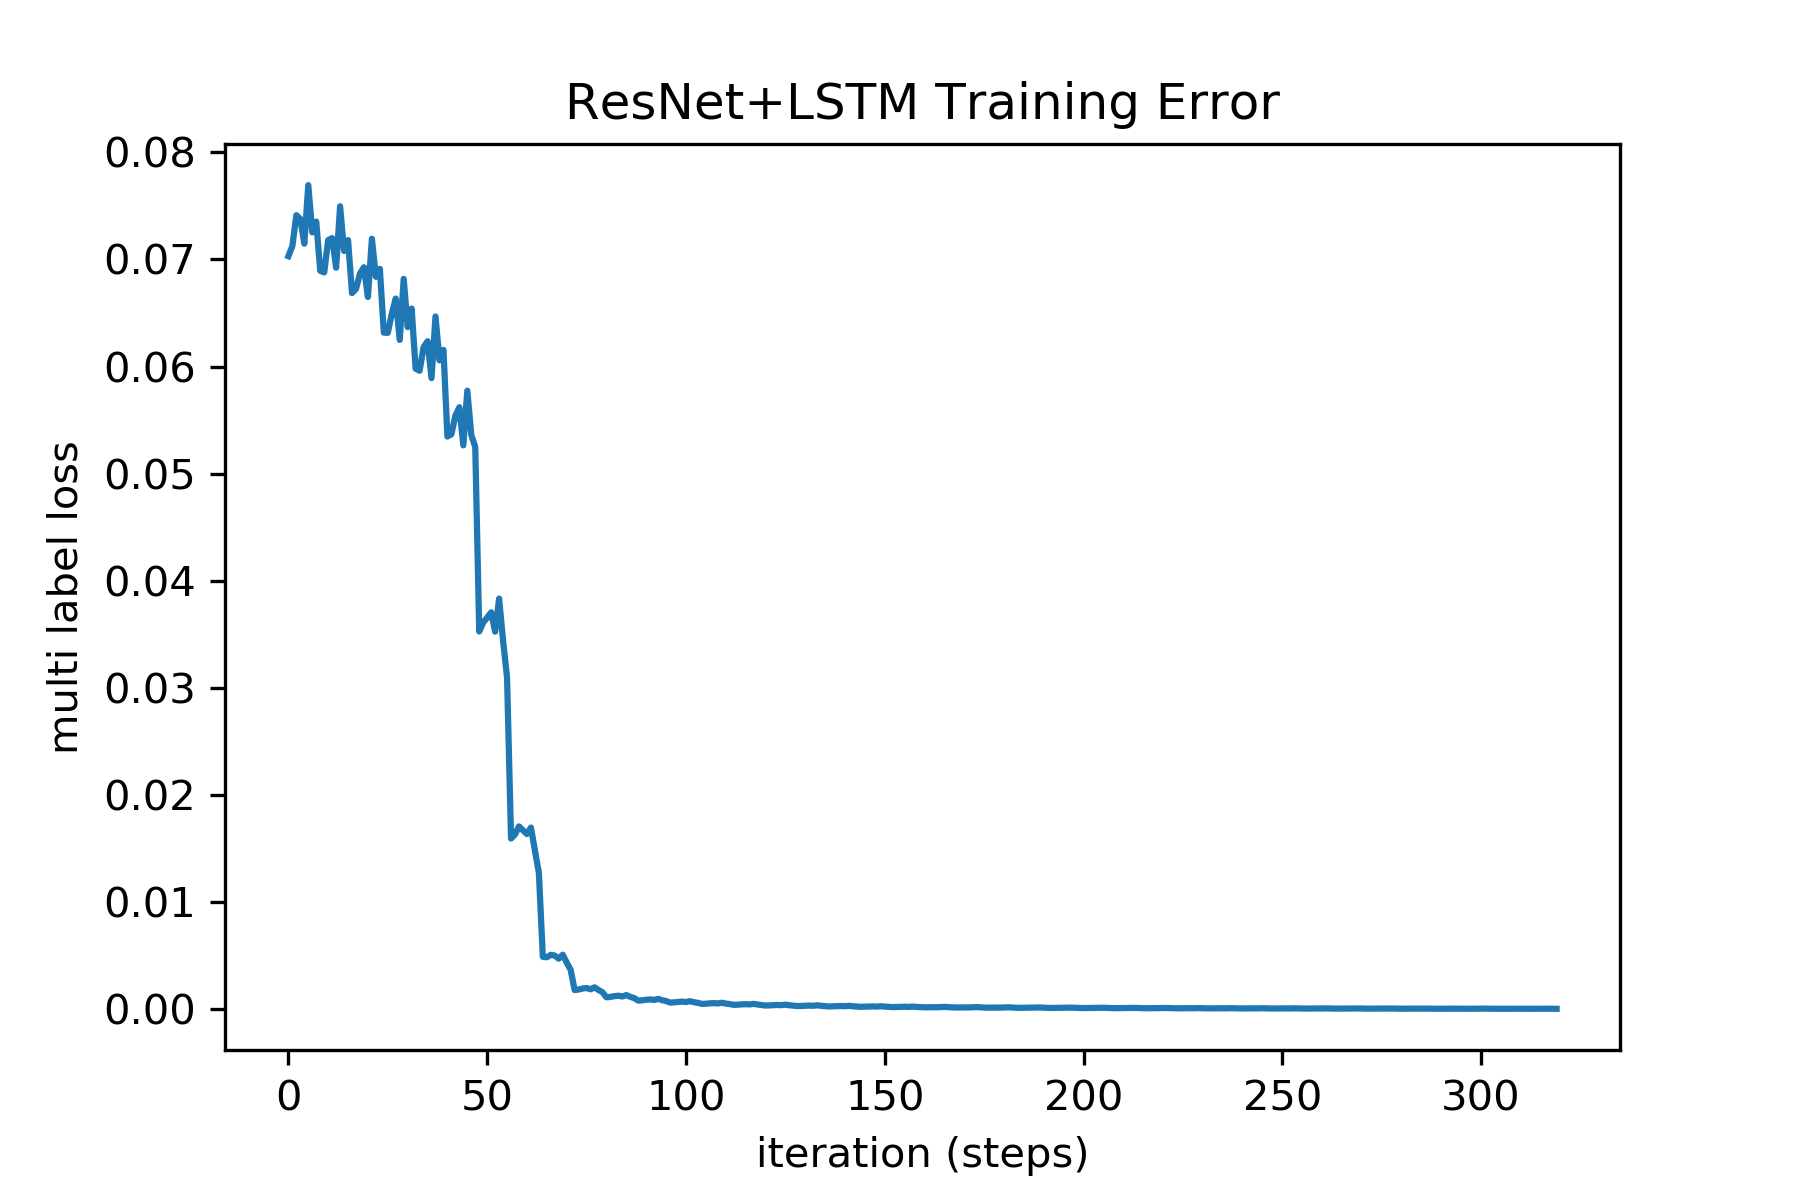
\includegraphics[width=1\linewidth]{./ResNet.png}
\end{center}

\begin{center}
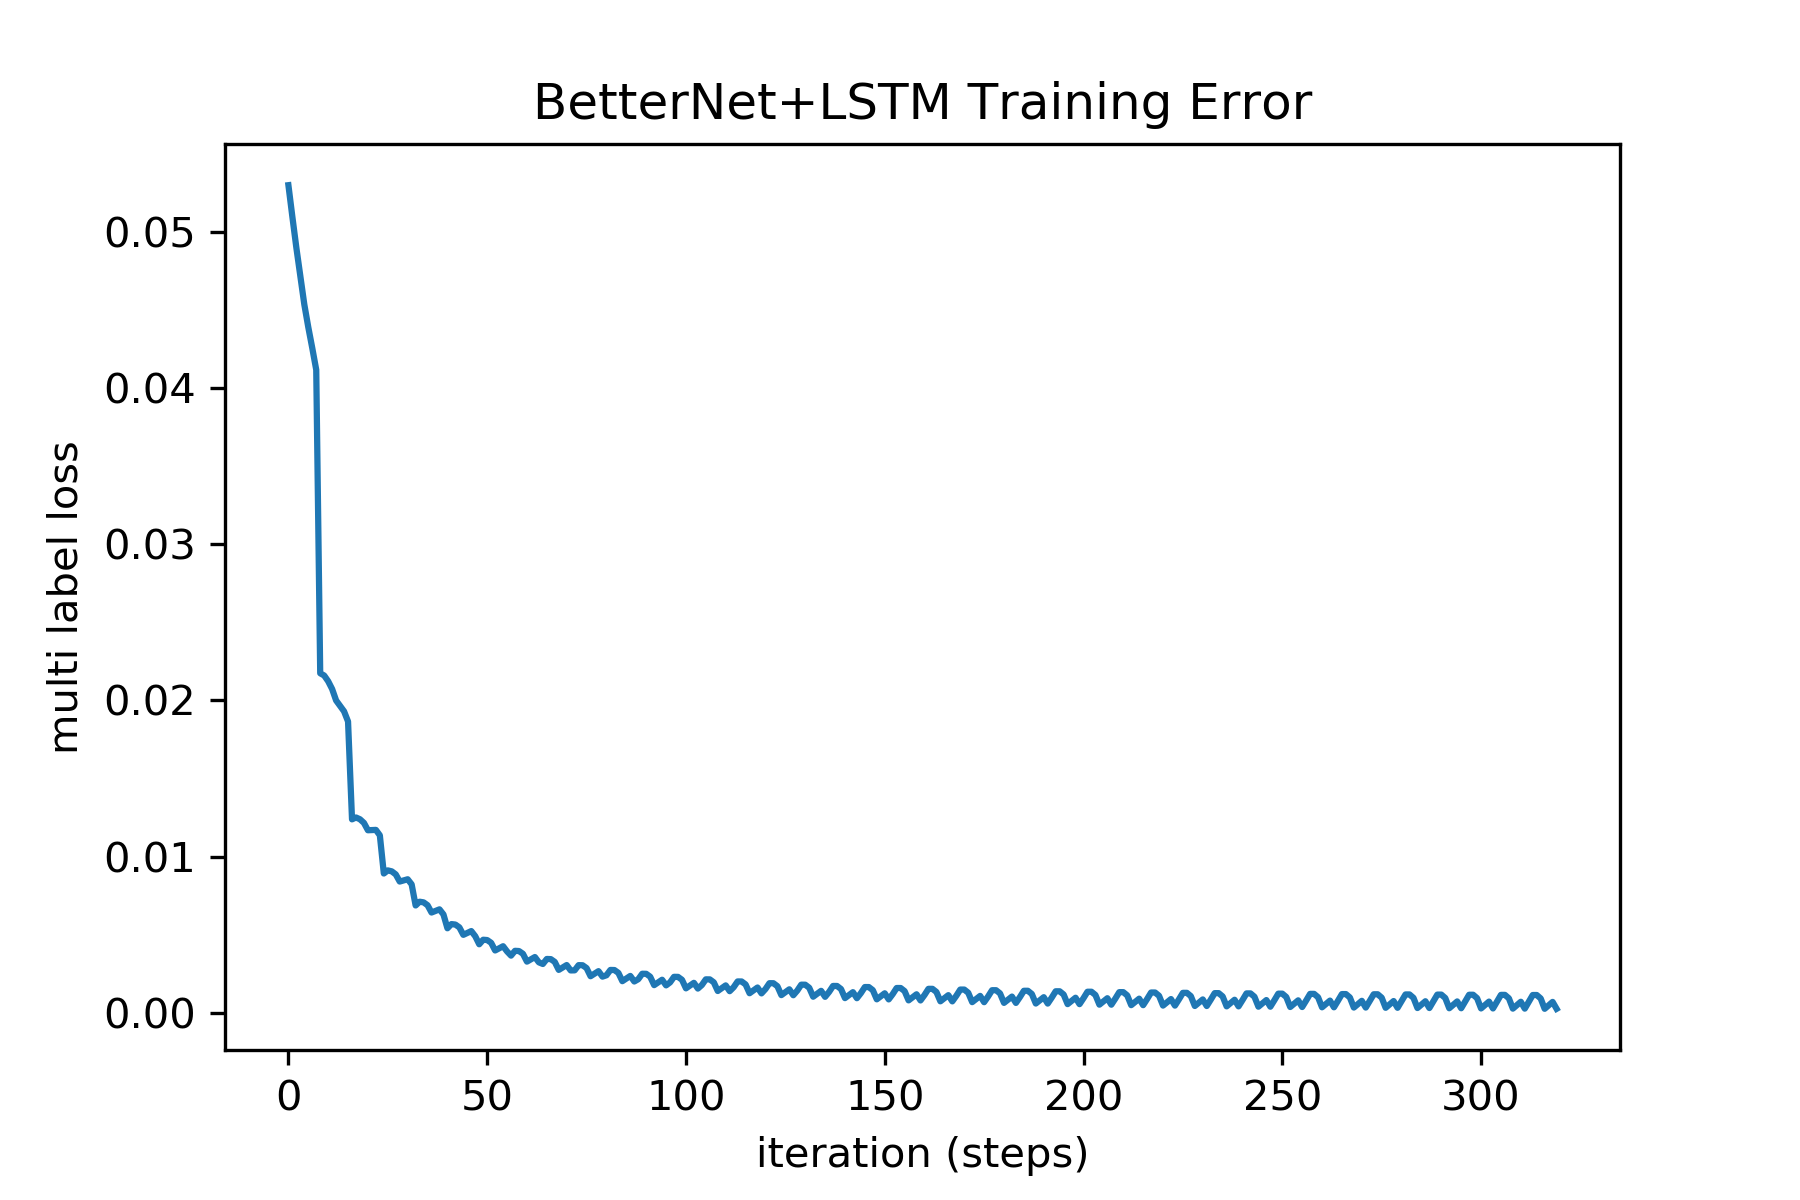
\includegraphics[width=1\linewidth]{./BetterNet+LSTM.png}
\end{center}

\subsection{Training Approach}
\texttt{BetterNet+LSTM} showed instantly decreasing training multi-label loss compared to \texttt{ResNet}. LSTM which performs teacher forcer learns temporal patterns from observation vectors again and again. After plotting the graphs with those two models, we concluded that \texttt{BetterNet+LSTM} is needed to have more complexity to learn more latent features of images, and higher tolerance to detect convergence of our model quickly.

\subsection{Test Approach}
We construct \texttt{BetterNet+LSTM} and tried to examine test aspect performance by varing many hyperparameters. Since LSTM modules take one-hot encoding captions as inputs, our model can easy find temporal patterns on CAPTCHA labels while training. However in test, foward algorithm in LSTM cell take those ground truth as inputs and \texttt{BetterNet+LSTM} trained test data even before comparison between predicted and true labels. By the approach, we found out the reason why our model performs 100.0\% test accuracy.

%-------------------------------------------------------------------------
\section{Conclusion}

We've selected ResNet and LSTM for CNN and RNN modules respectively. In result, \texttt{BetterNet+LSTM} shows fast and accurate performance while training, and predicted every label of test images correctly. However, we found out that we were testing our model while training and have to reconstruct the entire LSTM module. In future works, we'll rebuild our model which has forward algorithm not to take captions as inputs and train with numerous instances and diverse CAPTCHA examples. We'd like to extract more relevant features from the CNN module even when complexity reduction.

\begin{thebibliography}{9}

\bibitem{captcha} 
Adam Geitgey, ``How to break a CAPTCHA system in 15 minutes with Machine Learning", Dec. 2017

\bibitem{recaptcha} 
Adam Geitgey, ``The reCAPTCHA Project – Carnegie Mellon University CyLab". {\textit{www.cylab.cmu.edu. Archived}}, Jan. 2017

\bibitem{image-captioning} 
yunjey, ``Image Captioning", {\textit{GitHub pytorch-tutorial}}, Nov. 2018

\bibitem{adam} 
Diederik P. Kingma, Jimmy Ba, 
``Adam: A Method for Stochastic Optimization", {\textit{3rd International Conference for Learning Representations}}, San Diego, 2015



\end{thebibliography}
% [8] API Documentation of hmmlearn.MultinomialHMM (https://hmmlearn.readthedocs.io/en/latest/api.html#multinomialhmm)

\end{document}
